\documentclass[11pt,a4paper]{report}
\usepackage[a4paper,top=2.5cm,bottom=2.5cm,left=2cm,right=2cm]{geometry}
\usepackage[utf8]{inputenc}
\usepackage{amsmath}
\usepackage{amsfonts}
\usepackage{amssymb}
\usepackage{graphicx}
\usepackage{titlesec}
\usepackage{eurosym}
\usepackage{booktabs}
\usepackage{setspace}
\usepackage{wrapfig}
\usepackage{fancyhdr}
\usepackage{caption}
\usepackage{lipsum}
\usepackage{blindtext}
\usepackage{multicol}
\usepackage{array}
\usepackage{caption}
\usepackage{float}

\begin{document}

	\begin{center}
		\begin{onehalfspace}
			\par
			\textbf{UNIVERSITÀ DEGLI STUDI DI MILANO-BICOCCA} \\
			Scuola di Scienze \\
			Corso di laurea magistrale in Data Science
		\end{onehalfspace}
	\end{center}
	\smallskip
	\begin{center}
	
\includegraphics[width=2.78cm, height=2.96cm]{imgs/download.png}
\end{center}
	\begin{doublespace}
	\begin{center}
		{{{\LARGE \textbf{Data Management and Data Visualization project}}}}
	\end{center}
\end{doublespace}

	\smallskip
	
	\begin{doublespace}
		\begin{center}
			{{{\LARGE \textbf{Oscar's night analysis}}}}
		\end{center}
	\end{doublespace}




	\par
	\bigskip
	\bigskip
	\bigskip
	\bigskip
	\bigskip
	\bigskip
	\bigskip
	
	\bigskip
	\bigskip
	\bigskip
	\bigskip
	\bigskip
	\bigskip
	\vspace{8mm}
	\par
	
	\begin{flushleft}
		{\large \textbf{Corso condotto da:}  \\
			\textit{Prof. Federico Cabitza}\\
			\textit{Prof. Andrea Maurino}
		}
	\end{flushleft}
	
	\begin{onehalfspace}
		\begin{flushright}
			{\small \textbf{Gruppo di lavoro:} \\
				\textit{Claudio Fadda matr. 813499} \\
				\textit{Monica Vivace matr. 820470}}
		\end{flushright}
	\end{onehalfspace}
	
	
	\vfill
	\par
	\begin{center}
		{\large \textbf{Anno Accademico 2020-2021}}
	\end{center}
	
	
	\pagenumbering{gobble} % remove page numbering 

\begin{abstract}
Il 25 Aprile 2021 si è svolta la 93\textsuperscript{a} edizione dei premi Oscar, premio cinematografico più atteso e rinomato al mondo.
In questo elaborato si è cercato di esaminare il quadro generale della serata attraverso la raccolta di tweet in lingua inglese.
Lo \textbf{streaming} è stato svolto attraverso l'architettura \textit{Kafka}, mentre per lo \textbf{storing} è stato usato \textit{Apache NiFi} che ha consentito di trasferire tutti i tweet scaricati direttamente su \textit{MongoDB}.
La parte di \textbf{pre-processing} e di \textbf{integrazione} è stata svolta con \textit{Python}. L'integrazione è stata effettuata tra il dataset contenente i tweet e due database che contenevano informazioni sui film.
Per mostrare  i risultati del lavoro sono state create tre visualizzazioni che racchiudessero i punti focali del progetto sia per i film sia per gli/le attori/attrici, le visualizzazioni sono state create tramite il software \textit{Tableau}.
\end{abstract}
	\tableofcontents
	\cleardoublepage
	\pagenumbering{arabic}


\part{Data Management}



\chapter{Introduzione}
L'\textit{Academy Award}, conosciuto anche come Premio Oscar, è uno dei più antichi e prestigiosi premi cinematrografici. La cerimonia si svolge ogni anno a Los Angeles, città dove sorge il quartiere di Hollywood conosciuto per essere il fulcro dell'industria cinematografica.

I premi vengono conferiti dall'\textit{Academy of Motion Picture Arts and Sciences} (AMPAS) composta da persone che hanno avuto un ruolo chiave nel mondo del cinema.\\Per far in modo che un film venga candidato agli Oscar, deve rispettare una serie di requisiti imposti dall'AMPAS, regole abbastanza ferree, che per il 2021 sono state leggermente smorzate, infatti per la prima volta l'Academy ha consentito anche ai film trasmessi attraverso servizi streaming e/o on demand di poter essere ammessi alle candidature purché avessero una data di uscita ufficiale programmata nei cinema dopo la cerimonia degli Oscar. Tale deroga è stata rilasciata a causa del perdurare della pandemia da Covid-19 che ha dato un duro colpo all'industria cinematografica, sia durante lo svolgimento delle riprese dei film, sia per quanto riguarda la distribuzione degli stessi nelle sale cinematografiche, bloccata per le norme che imponevano la chiusura dei luoghi pubblici \cite{noauthor_academy_2021} \cite{noauthor_oscarsorg_nodate}.

A causa delle incertezze dovute alla pandemia da Coronavirus la 93\textsuperscript{a} cerimonia dei Premi Oscar è stata svolta due mesi in ritardo, ma nonostante la situazione l'Academy ha potuto svolgere in sicurezza l'evento.

\chapter{Obiettivo}
Il progetto nasce con la volontà di indagare quanto le persone parlino di un determinato film o di un attore/attrice candidati, quali siano le categorie più discusse e i trend dei tweet nel corso della serata; per fare questo abbiamo considerato due delle tre V dei Big Data: Velocità e Varietà.
\begin{quote}
    Chi vince l'Oscar è anche il più discusso? I film che vincono l'Oscar sono anche quelli più acclamati dalla critica? Gli attori che prendono la famosa statuetta sono anche i più popolari? Qual è la categoria più discussa?
\end{quote}
%L'obiettivo di questa ricerca è andare a capire se esiste una relazione tra numero di tweets dedicati ad un particolare film/attore e vincita dell'Oscar; oltre a vedere se un punteggio della critica alto è associato alla vincita dell'Oscar.
Abbiamo considerato le categorie strettamente legate ad attori e film, in particolare:
\begin{itemize}
    \item \textbf{Oscar al miglior attore} - \textit{Actor in a Leading Role};
    \item \textbf{Oscar al miglior attore non protagonista} - \textit{Actor in a Supporting Role};
    \item \textbf{Oscar alla miglior attrice
} - \textit{Actress in a Leading Role};
    \item \textbf{Oscar alla miglior attrice non protagonista} - \textit{Actress in a Supporting Role};
    \item \textbf{Oscar al miglior film d'animazione} - \textit{Animated Feature Film};
    \item \textbf{Oscar alla migliore fotografia} - \textit{Cinematography};
    \item \textbf{Oscar ai migliori costumi} - \textit{Costume Design};
    \item \textbf{Oscar al miglior montaggio} - \textit{Film Editing};
    \item \textbf{Oscar al miglior film in lingua straniera} - \textit{International Feature Film};
    \item \textbf{Oscar alla migliore colonna sonora} - \textit{Music (Original Score)};
    \item \textbf{Oscar al miglior film} - \textit{Best Picture};
    \item \textbf{Oscar alla migliore scenografia} - \textit{Production Design};
    \item \textbf{Oscar al miglior sonoro} - \textit{Sound};
    \item \textbf{Oscar ai migliori effetti speciali} - \textit{Visual Effects};
    \item \textbf{Oscar alla migliore sceneggiatura non originale} - \textit{Writing (Adapted Screenplay)};
    \item \textbf{Oscar alla migliore sceneggiatura originale} - \textit{Writing (Original Screenplay)};
\end{itemize}

Abbiamo inoltre acquisito il punteggio fornito dalla critica (rating) e la popolarità determinata dagli utenti dal sito The Movie Database TMDB \cite{noauthor_tmdb_nodate}.

\chapter{Data Collection}
La raccolta dati è stata svolta attraverso il social network Twitter usando le API che la società mette a disposizione degli utenti per effettuare \textit{streaming} dei dati. Tramite l'architettura Kafka è stato possibile eseguire lo streaming creando dei particolari \textit{topic}; è stato realizzato anche un flusso con NiFi in modo da poter effettuare direttamente lo \textit{storage} su MongoDB.
Per tutta la parte di Data Collection si è fatto uso delle Virtual Machine Azure.

\section{Kafka, NiFi e MongoDB}
Lo \textit{streaming} dei tweet è stato processato attraverso la piattaforma Apache Kafka, un sistema di messaggistica che usa una struttura di \textit{publish}/\textit{subscribe}, permettendo ai \textit{producer} di inviare dati a determinati \textit{topic} di interesse, mentre ai \textit{consumer} di mettersi in ascolto su questi ultimi e ricevere i dati in arrivo. 

L'accesso alle API di Twitter viene reso disponibile attraverso la libreria Tweepy, creando un opportuno client di autenticazione che necessita dei quattro token (consumer key, consumer secret, access token, access secret) che Twitter mette a disposizione dei developer.

Per tenere il controllo dei dati in \textit{real time} si è fatto uso di un mini-flusso su Apache NiFi con il quale è stato possibile effettuare direttamente il salvataggio della coda dei tweet su MongoDB in formato JSON.

\section{Streaming}
Per scaricare i tweet durante la serata sono stati creati due topic indipendenti: un topic relativo agli attori/attrici ed un altro relativo invece ai film. Per entrambi i topic si è fatto uso del metodo “on\_status" offerto da Tweepy, attraverso questo metodo abbiamo scelto di scaricare per ogni tweet i seguenti attributi:
\begin{itemize}
\item \textit{date}
 \item \textit{user\_id}
 \item \textit{username}
 \item \textit{screen\_name}
 \item \textit{text}
 \item \textit{hashtags}
\end{itemize}
Inoltre, attraverso un controllo sull'attributo “extended\_tweet" si è richiesto di scaricare oltre ai tweet di lunghezza classica (140 caratteri) anche quelli con un numero di caratteri superiore (sino a 280 caratteri).

I tweet sono stati scaricati in base a delle keywords, usando il parametro “track" di filter, che permette appunto di scaricare quei tweet che contengono le parole chiave inserite nel parametro. Sono state inserite delle parole chiave che richiamassero i film, oppure nomi e cognomi degli attori candidati. In ogni caso qualsiasi keywords è stata usata insieme alla parola chiave “Oscars" in modo che fossero scaricati solo tweets inerenti la cerimonia.

Infine, tramite Apache NiFi, sono stati realizzati due piccoli flussi tramite dei processors chiamati “ConsumeKafka" e “PutMongoRecord" impostati in modo da sottoscrivere i due topics precedenti, ricevere i tweet e salvarli su due database MongoDB distinti.
	\begin{figure}[h]
			\centering
			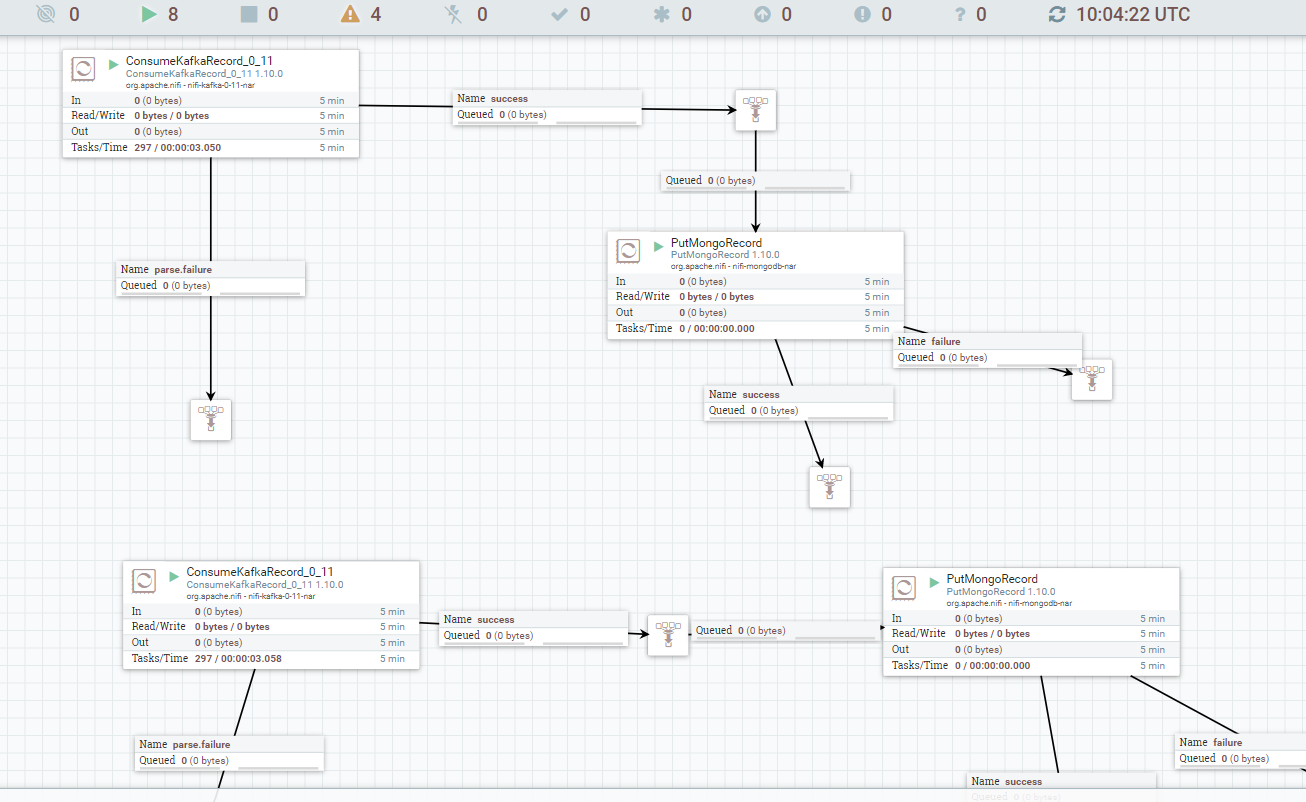
\includegraphics[width=0.8\linewidth]{imgs/NiFiImmagine.png}
			\caption{Flussi su Apache NiFi}
			\label{fig:Flussi su Apache NiFi}
		\end{figure}
\section{Database}
Alla fine del processo di \textit{streaming} sono stati ottenuti due database, uno relativo ai tweets scaricati sull'ambito dei film e un secondo ottenuto dai tweets relativo ad attori/attrici, rispettivamente di (153.716 e 145.525 righe), entrambi in formato JSON.

Successivamente i due database sono stati scaricati in locale in modo da poter essere elaborati in Python.
\chapter{Struttura dei dati}
\section{Dataset acquisiti tramite streaming}
Lo streaming dei dati ha permesso di ottenere due database così costituiti:
\begin{itemize}
 \item \textit{\_id}: un identificativo univoco che viene creato in maniera automatica da MongoDB;
 \item \textit{user\_id}: id numerico che identifica l'utente attraverso Twitter;
 \item \textit{username}: nome completo del profilo;
 \item \textit{screen\_name}: identificativo del nome utente su Twitter;
\item \textit{text}: testo del tweet;
 \item \textit{hashtags}: hashtags usati nel testo.
\end{itemize}

	\begin{figure}[h]
			\centering
			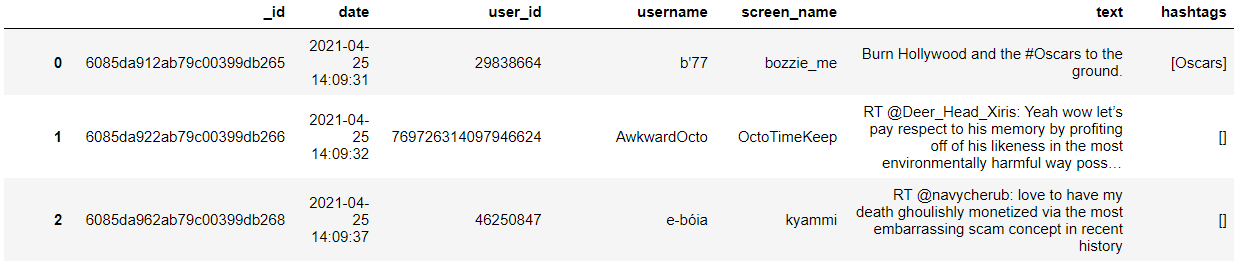
\includegraphics[width=0.9\linewidth]{imgs/struttura dataset.png}
			\caption{Struttura dataset}
			\label{fig:Struttura dataset}
		\end{figure}
\section{Dataset acquisiti per la varietà}
Per integrare i dati raccolti tramite lo streaming sono stati scelti dei dataset disponibili sul sito Kaggle, in particolare si è deciso di utilizzare un dataset proveniente da Internet Movie Database (IMDb) e due dataset provenienti da The Movie Database (TMDB) \cite{noauthor_imdb_nodate} \cite{noauthor_tmdb_nodate-1} \cite{noauthor_tmdb_nodate}.

\chapter{Pre processing}
Per manipolare i dati ottenuti tramite Twitter abbiamo usato il linguaggio Python e diverse librerie fra le quali: \textit{Pandas}, \textit{Difflib}, \textit{Re}, \textit{Datetime}, \textit{Emoji}.

Ogni membro del gruppo, avendo effettuato la raccolta dati in streaming, ha ottenuto due dataset uno durante il pre serata e uno durante la serata, quindi è stato deciso di inglobare i dataset relativi ai film in uno solo. Questa scelta è stata fatta in modo da avere un dataset unico, arricchito con i tweet mancanti sfuggiti allo streaming del singolo utente. Lo stesso procedimento è stato effettuato per il dataset relativo agli/alle attori/attrici. 

Dopo questa prima manipolazione, si è proceduto attraverso l'operazione di \textit{data cleaning}, alla pulizia dei dati acquisiti. In particolare, ci siamo concentrati sulla colonna del nostro dataset relativa al testo del tweet (text), questo dato per noi è molto importante perché nel testo sono presenti le parole chiave usate per fare streaming dei dati; la nostra idea infatti è stata quella di filtrare i soli tweet contenti citazioni a titoli di film in modo da poter capire successivamente quanto il film fosse stato discusso durante la serata. Sono state così eliminate le emoji, vari simboli (come quello di newline) e i link. Per poter raggiungere l'obiettivo sopra è stata costruita una funzione ad hoc che cerca all'interno del testo i titoli di film e li inserisce in una nuova colonna, in tal modo è stato possibile contare per ciascun film i tweet associati a esso, in modo da avere una stima diretta sull'apprezzamento di ognuno dal pubblico.

Inoltre è stata effettuata una importante modifica in relazione agli orari di pubblicazione dei tweet. L'attributo “date" è legato alla timezone UTC +0, considerando questa informazione in aggiunta al fatto che in Italia nel mese di aprile sia in vigore l'ora solare e che la differenza rispetto a Los Angeles è dì 9 ore, si è reso quindi necessario effettuare una modifica per un totale di -7 ore all'attributo “date" così da allineare l'orario dei tweet e quello degli avvenimenti durante la Notte degli Oscar.

Questi procedimenti sono stati eseguiti anche per il dataset relativo agli attori/attrici.

I dataframe ottenuti sono i seguenti:

	\begin{figure}[h]
			\centering
			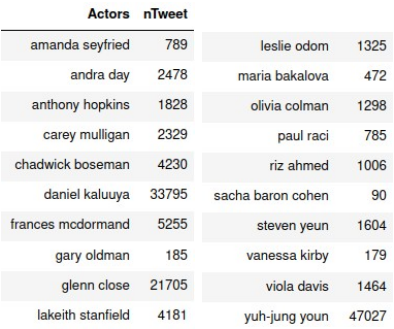
\includegraphics[width=0.30\linewidth]{imgs/actrs.png}
			\caption{Numero di tweet per attori/attrici}
			\label{fig:Prima infografica}
		\end{figure}

	\begin{figure}[h]
			\centering
			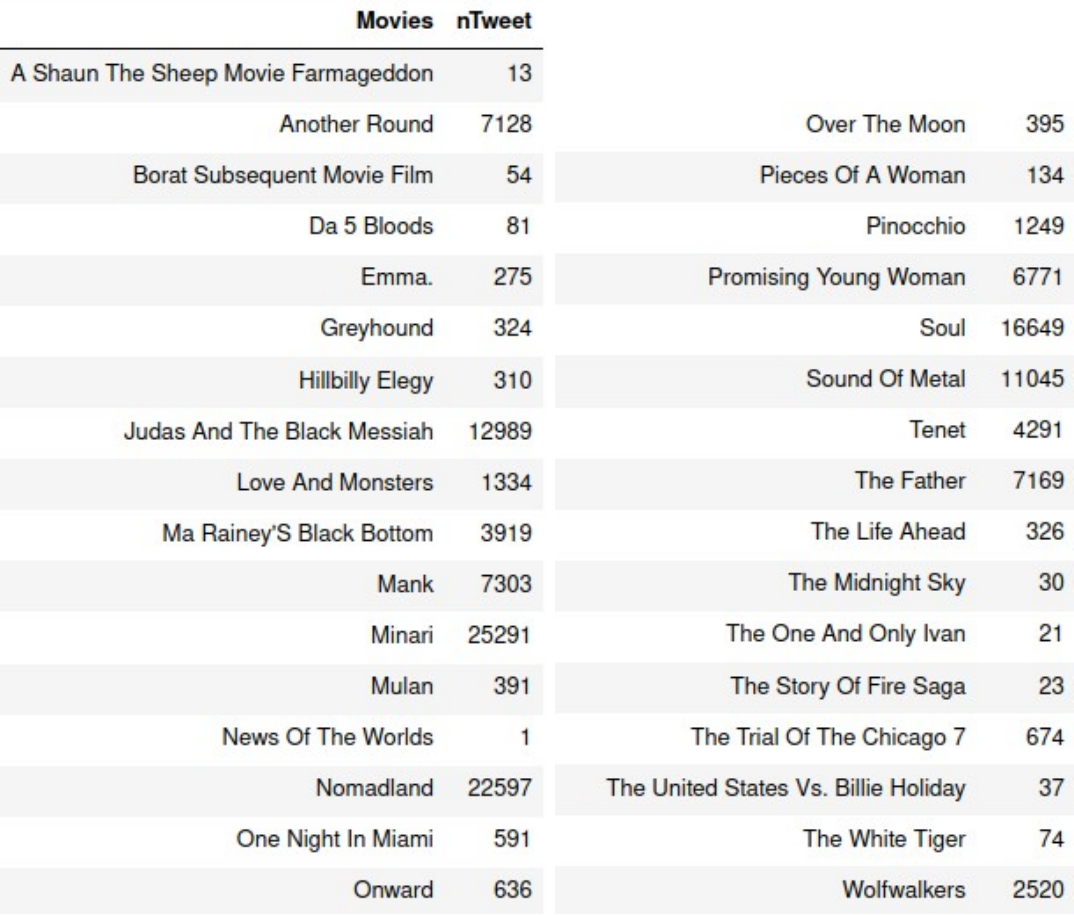
\includegraphics[width=0.40\linewidth]{imgs/movies.png}
			\caption{Numero di tweet per film}
			\label{fig:Prima infografica}
		\end{figure}

\newpage		
E' da segnalare un nostro errore nella compilazione delle keywords utilizzate per lo streaming. Le keywords relative al film “News of the World" presentano un errore di battitura, come si può vedere dalla Figure 5.1, è stata inserita erroneamente una “s" alla fine della parola “World" causando quindi l'impossibilità di scaricare correttamente i tweet di nostro interesse.

\chapter{Descriptive Analysis}
Svolgendo un'analisi descrittiva dei dataset emergono informazioni interessanti. 

\begin{table}[h]
	\begin{center}
	\begin{tabular}{ccc}
		\toprule
		          & Tweet totali & Retweet totali \\
		\midrule
	Attori/Attrici - Pre & 145.525 & 114.381  \\
	Movies - Pre & 153.716 & 108.065 \\
	\end{tabular}
	\caption{Numero di tweet e retweet pre eliminazione degli utenti bot}
	\label{descrittiva}  
		\end{center} 
\end{table}

Dai dati si vede che sia per i film, sia per gli/le attori/attrici buona parte dei tweet è rappresentata da Retweet e questo è visibile in modo più immediato dai grafici \ref{fig:Tweet vs Retweet attori/attrici} e \ref{fig:Tweet vs Retweet film}.

	\begin{figure}[h]
			\centering
			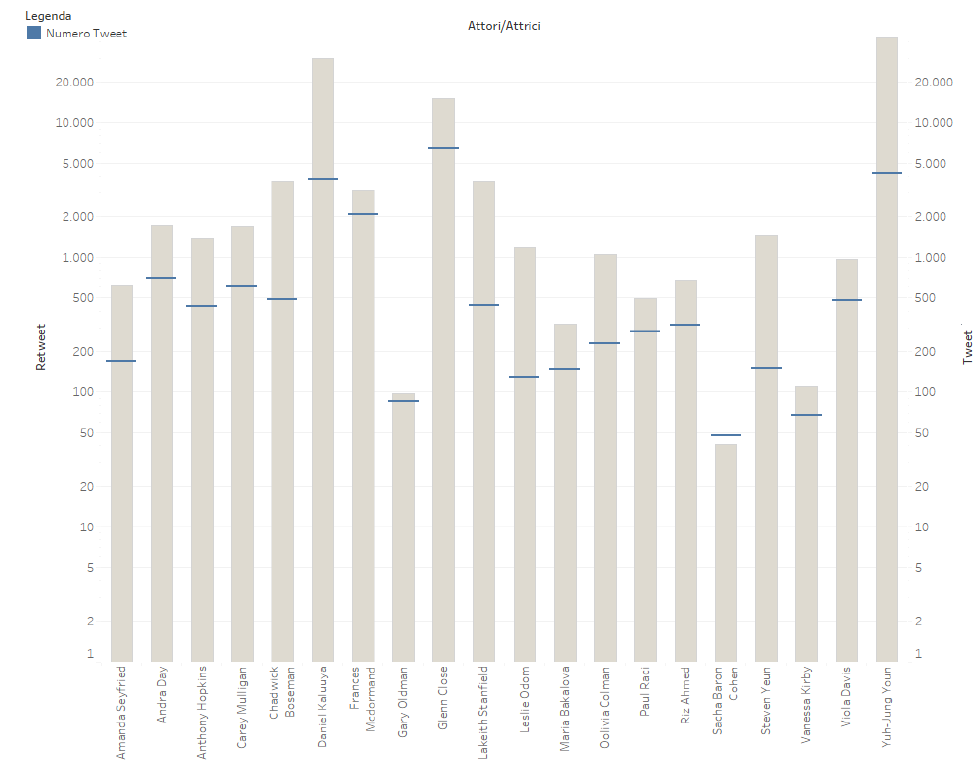
\includegraphics[width=0.7\linewidth]{imgs/actors111.png}
			\caption{Tweet vs Retweet attori/attrici}
			\label{fig:Tweet vs Retweet attori/attrici}
		\end{figure}

	\begin{figure}[h]
			\centering
			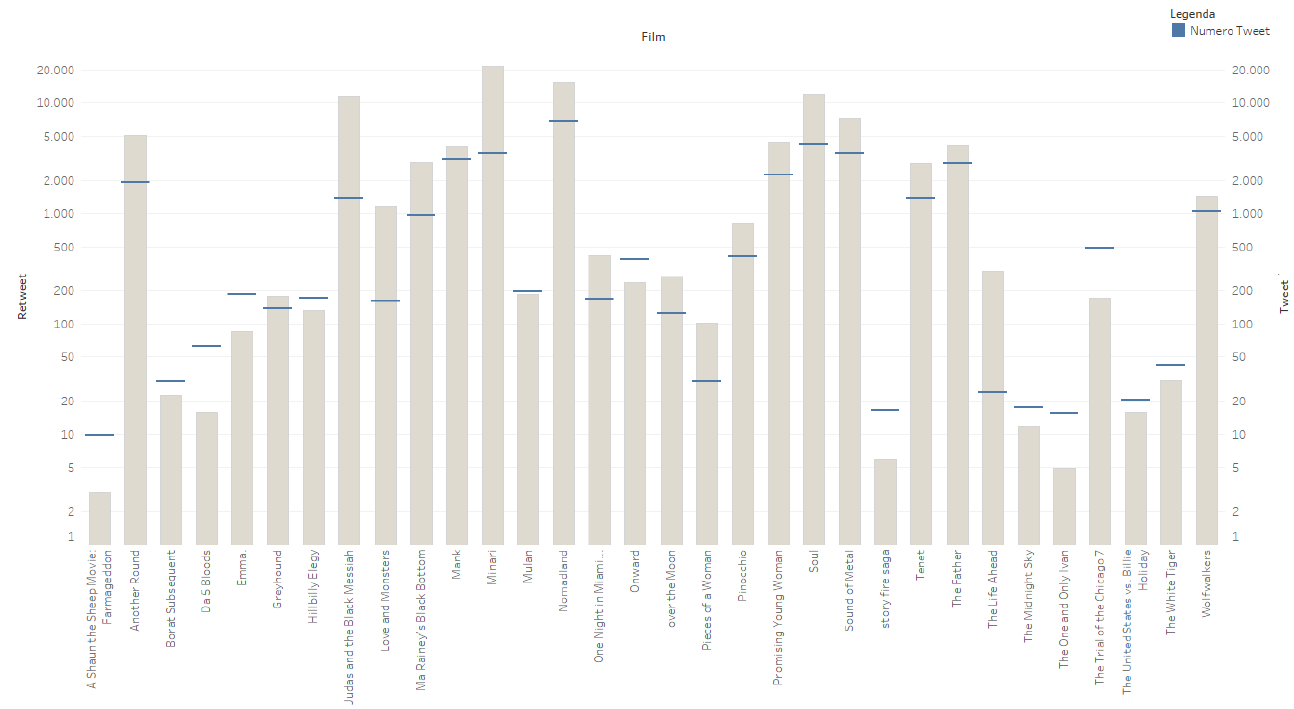
\includegraphics[width=0.9\linewidth]{imgs/movie.png}
			\caption{Tweet vs Retweet film}
			\label{fig:Tweet vs Retweet film}
		\end{figure}

Tra i fatti interessanti emersi durante l'analisi dei dataset si nota in primo luogo la presenza di tweet senza alcuna menzione ai film e questi costituiscono circa il 17\% del dataset film. In secondo luogo si nota la presenza di tweet pubblicati nello stesso secondo e con medesimo testo, indice del fatto che potrebbero essere stati creati da utenti bot, questi ultimi sono pari a 35 e complessivamente hanno creato circa 375 tweet durante l'intero evento. Ulteriore fattore da prendere in considerazione è la presenza di utenti che pubblicano un numero di tweet eccessivamente alto durante la giornata, generalmente si tende a considerare bot quegli utenti che pubblicano più di 75 tweet al giorno, poiché risulta pressoché improbabile pubblicare una media di un tweet ogni quarto d'ora. Tuttavia nel primo caso tali utenti sono stati eliminati poiché non è possibile pubblicare più tweet nello stesso secondo, nel secondo caso invece i presunti bot non sono stati eliminati perché rappresentavano soltanto una piccola percentuale della totalità di utenti (circa lo 0.03\%). 

Per il dataset attori vale il medesimo discorso, nello specifico i tweet che non presentano menzione di attori/attrici costituiscono il 22\% del dataset, gli utenti che pubblicano invece nel medesimo momento sono pari a 41 ed i tweet pubblicati sono complessivamente 264. Per ciò che concerne invece gli utenti a cui è associato un alto numero di tweet pubblicati in questo caso rappresentano lo 0.01\% del totale. 

I numeri rilevati a seguito di eliminazione dei tweet pubblicati dagli utenti bot sono i seguenti: 
\begin{table}[h]
	\begin{center}
	\begin{tabular}{ccc}
		\toprule
		          & Tweet totali & Retweet totali \\
		\midrule
	Attori/Attrici - Post & 121.493 & 110.258  \\
	Movies - Post & 126.737 & 97.880 \\
	\end{tabular}
	\caption{Numero di tweet e retweet post eliminazione degli utenti bot}
	\label{descrittiva}  
		\end{center} 
\end{table}

\chapter{Data Integration}
L'integrazione, come precedentemente indicato, è stata svolta attraverso dei dataset estratti dal sito IMDB e TMDB, siti che contengono un gigantesco archivio di informazioni sul cinema.

Questi dataset contengono al loro interno una chiave esterna molto importante, che identifica in modo univoco un singolo film, chiamata “imdb\_id"; questa chiave è stata usata per filtrare la miriade di dati contenuti al loro interno, permettendo di individuare i film per noi rilevanti, ovvero quelli candidati agli Oscar 2021. Dopo aver ridotto la dimensione dei dataset si è proceduto con la \textit{data enrichment} in modo da valutare eventuali incongruenze tra le stesse informazioni ed aggiungere nuove informazioni rilevanti; particolare attenzione è stata posta per alcune colonne che contenevano al loro interno dei documenti json annidati, che sono stati estratti e rappresentati come dataframe individuali. E' stata necessaria anche una fase di pulizia dei dati, in quanto sono stati riscontrati alcuni errori sui database.

Un'informazione importante per il nostro progetto è il rating che ogni film ha ottenuto dalla critica. Nel nostro caso abbiamo deciso di scegliere come punteggio quello che è stato dato dalla piattaforma TMDB, questo perché risultava essere l'unico a contenere tutti i film da noi menzionati.

Allo stesso modo è stata eseguita l'integrazione relativa agli/alle attori/attrici, anche in questo caso abbiamo scelto come piattaforma di riferimento TMDB, che nel database conteneva anche informazioni relative al cast di ogni film e al regista. A ciascuno di essi era inoltre associata una chiave univoca che identifica un particolare attore. La chiave ci ha permesso di risalire all'attributo “Popularity" ossia la popolarità di ogni artista contenuta in un file differente. Questo attributo viene calcolato da TMDB prendendo in considerazione il numero di visite degli utenti durante la giornata sul profilo dell'attore/attrice e il punteggio ottenuto come popolarità nei giorni precedenti.

\chapter{Risultati}
L'integrazione fra i diversi dataset ha permesso la costruzione di sei visualizzazioni che sono state estremamente utili per poter trarre delle conclusioni e rispondere alle iniziali domande di ricerca (le visualizzazioni sono visibili al link in fondo al report). Nello specifico dalle prime due infografiche \ref{fig:Prima infografica} che mostrano l'andamento dei tweet durante la Notte degli Oscar si rileva una corrispondenza tra i picchi e l'effettiva premiazione, anche se talvolta sono presenti picchi che non sembrano avere corrispondenza o viceversa non sono presenti picchi rilevanti in caso di vincita, si veda ad esempio Anthony Hopkins che ha vinto il premio come “Best Actor" senza tuttavia ottenere un consenso da parte del pubblico. Nella terza e quarta infografica che consentono un confronto fra quanto è stato discusso un film (attore/attrice) e il punteggio ottenuto dalla critica (popolarità) emerge una corrispondenza fra i film vincitori e un alto valore del rating (es. Soul, The Father, Sound of Metal, Tenet). Lo stesso si può dire per ciò che concerne gli/le attori/attrici. Infine dalla quinta e sesta infografica che mostrano le categorie più discusse dal pubblico a fine serata si può notare che la categoria più discussa è “Best Picture" per ciò che concerne i film mentre per ciò che concerne attori/attrici le categorie più discusse sono “supporting role" maschile e femminile. Si nota inoltre che le attrici hanno raccolto un maggior numero di tweet rispetto agli attori. 


\chapter{Conclusioni e sviluppi futuri}
Dopo aver applicato diversi strumenti per svolgere processamento, pulizia, integrazione e arricchimento dei dati, si possono evidenziare diversi problemi sorti durante le diverse fasi. Una delle problematiche deriva dai dati stessi che ne hanno resa complessa la manipolazione a causa della presenza di emoji, simboli non solo all'interno del testo del tweet ma anche nello Username e nello ScreenName. Altro problema sorto durante la manipolazione deriva dalla presenza di alcuni Retweet troncati che non hanno permesso una loro valutazione, questo fattore dovrebbe essere pertanto preso in considerazione in analisi future. Ulteriore problema sorto e di cui si è già ampiamente parlato sopra riguarda la presenza di tweet che non menzionavano alcun film/attore/attrice, si incentiva pertanto chi vorrà fare una analisi futura a prestare particolare attenzione durante la fase di streaming.


\part{Data Visualization}

\chapter{Infografiche}
\section{Tweet trend and award winners - Movies \& Actors/Actress}
Le prime due infografiche mostrano l'andamento dei tweet durante la Notte degli Oscar e hanno permesso di rispondere alla prima delle tre domande di ricerca: “Chi vince l'Oscar è anche il più discusso?".  

	\begin{figure}[h]
			\centering
			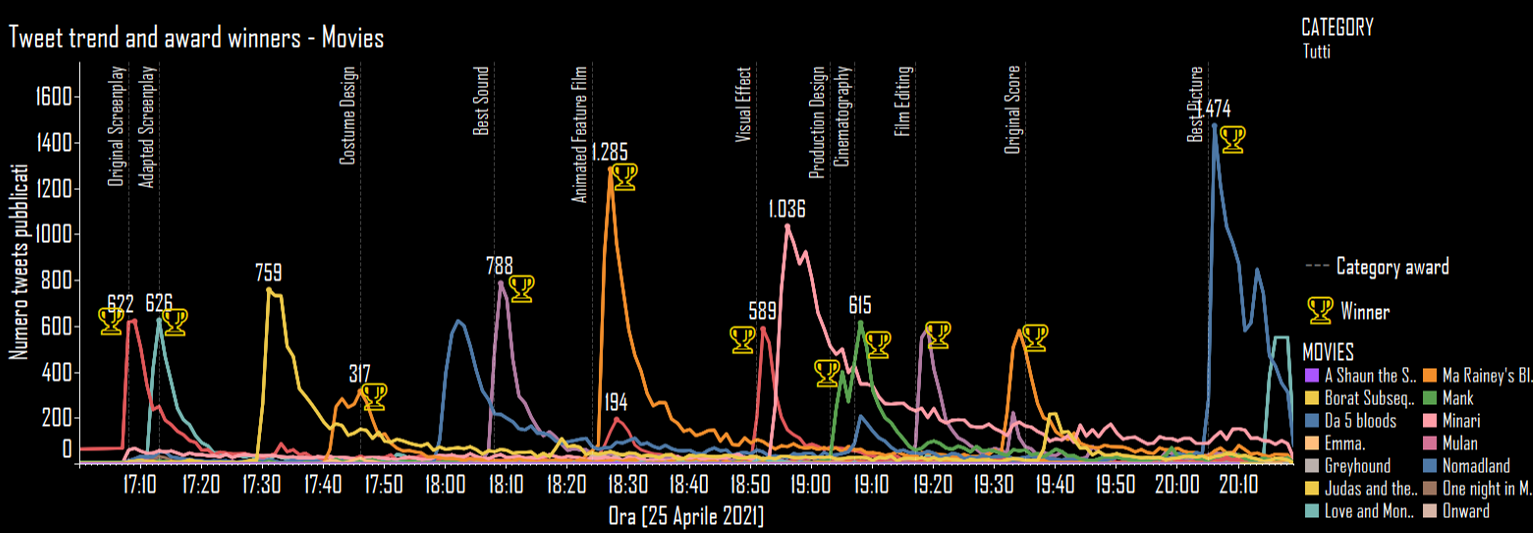
\includegraphics[width=1\linewidth]{imgs/INFOGRAFICA1.png}
			\caption{Prima Infografica}
			\label{fig:Prima infografica}
		\end{figure}


Nello specifico abbiamo raggruppato i film e gli attori per categorie a cui sono stati nominati. L'aggiunta delle linee tratteggiate che rappresentano il momento della premiazione permettono di avere una visione completa dell'evento. Al candidato vincitore è associata una coppa che indica la vittoria per la categoria specifica.

Per quanto concerne la domanda di ricerca possiamo affermare che esista una corrispondenza dei picchi con l'effettiva premiazione, ma sono visibili anche ulteriori picchi che apparentemente non sembrano avere corrispondenza. Confrontando la prima infografica con la seconda si evince che i picchi “anomali" nell'infografica relativa ai film corrispondono alle premiazioni degli attori e derivano dal fatto che insieme al nome dell'attore è stato tweettato anche il titolo del film associato. 

Merita un discorso a parte invece il picco delle 19:50 circa relativo a Glenn Close (seconda infografica). In quel momento della serata infatti si è verificato un siparietto comico che ha coinvolto l'attrice portando un focus del pubblico su tale avvenimento che ha quindi generato un incremento di tweet.

In generale quindi risulta esserci una certa aderenza tra chi vince l'Oscar e il “picco di discussione" avvenuto su Twitter; possiamo anche notare però quanto avvenuto nel caso di Anthony Hopkins che ha vinto il premio come “Best Actor" ed ha effettivamente ottenuto un picco a seguito della premiazione ma tale picco risulta estremamente inferiore rispetto agli altri, avvenimento che ci possiamo spiegare a seguito del fatto che la vincita dell'attore non è stata accompagnata da un gradimento da parte del pubblico.

\section{Rating (TMDB) vs count tweets - Movies \& Actors/Actress}

La terza e la quarta infografica consentono un confronto fra quanto è stato discusso un film (attore/attrice) e il punteggio ottenuto dalla critica (popolarità), tuttavia rispetto alle visualizzazioni precedenti i tweet sono stati raggruppati in fasce orarie (attraverso una aggregazione ogni 30 minuti).  La realizzazione di queste ultime ha permesso di rispondere alla seconda e alla terza domanda di ricerca: “I film che vincono l'Oscar sono anche quelli più acclamati dalla critica? Gli attori che prendono la famosa statuetta sono anche i più popolari?". 

	\begin{figure}[h]
			\centering
			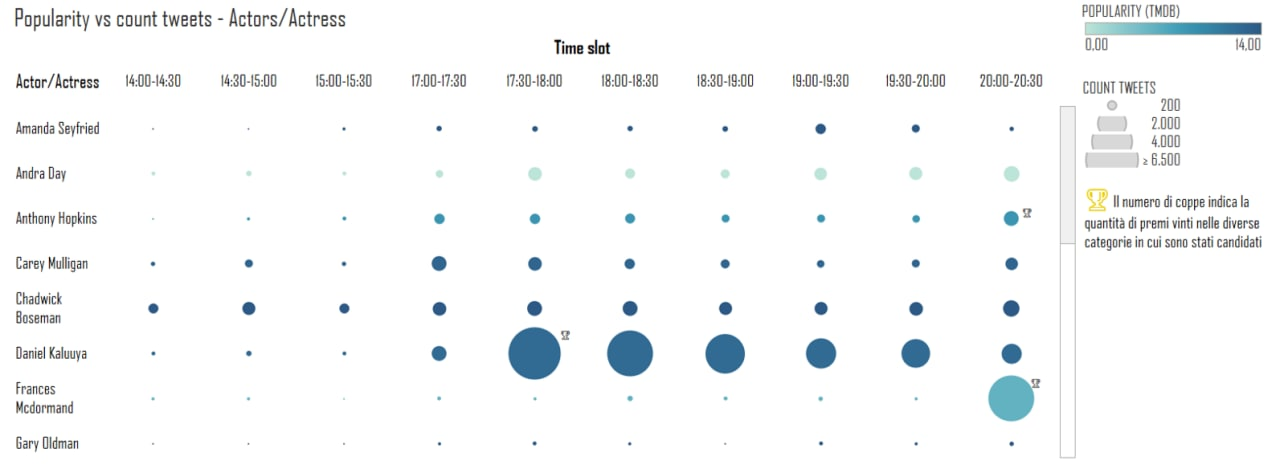
\includegraphics[width=1\linewidth]{imgs/photo1631116691.jpeg}
			\caption{Terza Infografica}
			\label{fig:Terza infografica}
		\end{figure}

  Per ciò che riguarda i film si nota una corrispondenza fra i film vincitori e un alto valore del rating, si vedano ad esempio i film Soul, The Father, Sound of Metal, Tenet. Un'eccezione è invece rappresentata dal film Wolkwalkers che pur ottenendo un rating pari a 8.5 non ha ottenuto alcun Oscar. Per ciò che concerne gli/le attori/attrici si nota una quasi totale corrispondenza tra vincita dell'Oscar e alti valori di dellla popolarità ad eccezione dell'attrice Yuh Jung Joun che non presentava alcun rating sulla piattaforma TMDB, va notato infatti che nonostante l'attrice avesse già partecipato a dei film per il mercato orientale, il film Minari ha sancito il suo debutto su quello occidentale.

\newpage
\section{Movies Categories \& Actors/Actress Categories}
Anche in questo caso sono state create due infografiche che andassero a mostrare a fine serata, quale è stata (o sono state) la categoria più discussa dal pubblico. In questo caso il trend dei tweet è stato costruito mediante un'aggregazione degli stessi per categoria. 

	\begin{figure}[h]
			\centering
			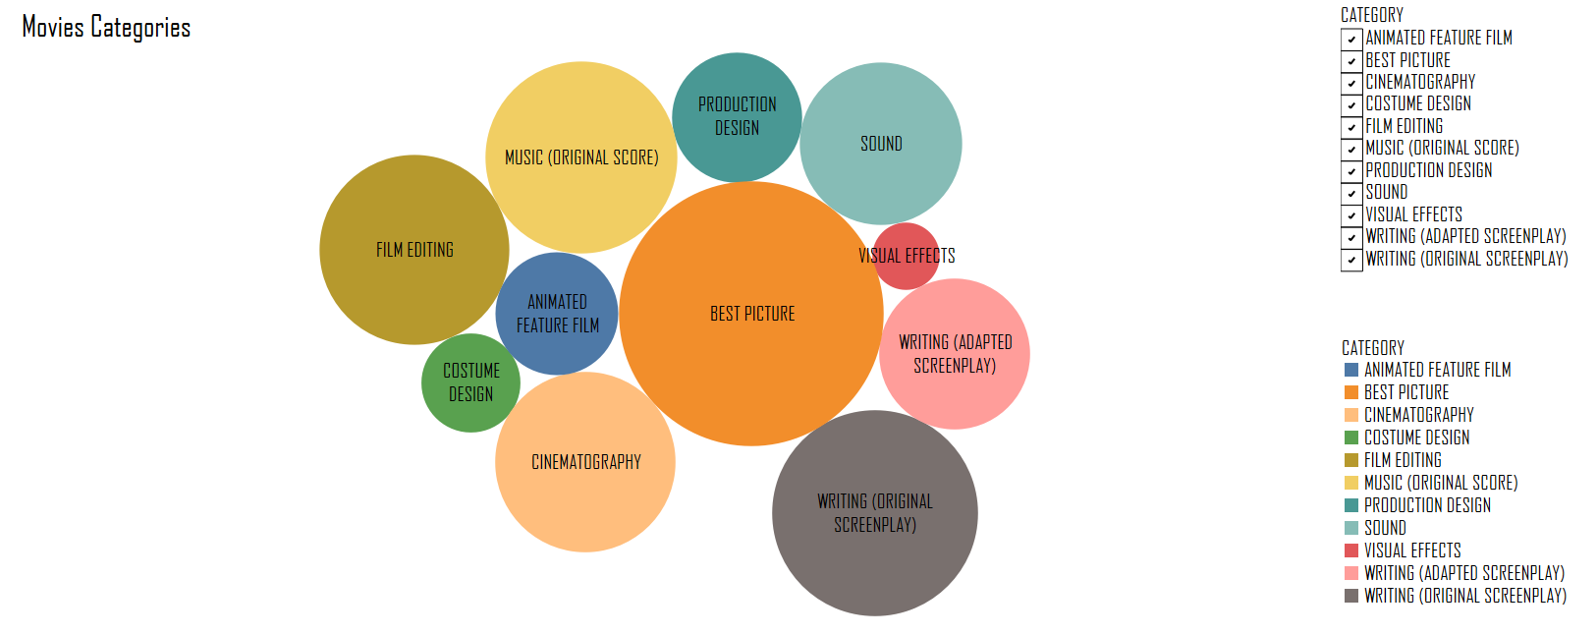
\includegraphics[width=1\linewidth]{imgs/Infografica5OKOK.png}
			\caption{Quinta Infografica}
			\label{fig:Terza infografica}
		\end{figure}
		
La quinta infografica mostra come la categoria più discussa relativa ai premi per i film sia “Best Picture", questo non sorprende in quanto questa categoria è la più ambita e importante.
La sesta infografica invece, ci permette di apprezzare un dato sorprendente: le categorie corrispondenti ai “supporting role" maschile e femminile sono stati maggiormente discussi rispetto ai “leading role", fatto interessante visto che il “supporting role" era storicamente considerato meno rilevante.
Infine, si nota anche che per quanto riguarda attori e attrici, queste ultime hanno raccolto un maggior numero di tweet rispetto agli attori.

\chapter{Valutazione della qualità}
Per la valutazione della qualità delle infografiche è stata svolta:
\begin{itemize}
 \item \textit{Valutazione euristica};
 \item \textit{Questionario psicometrico};
 \item \textit{User test}.
\end{itemize}

\section{Valutazione euristica}
La valutazione euristica è stata sottoposta a tre persone; i soggetti hanno potuto interagire liberamente con le visualizzazioni senza svolgere dei task specifici ma con la sola richiesta di parlare a voce alta in modo da capire quali fossero le difficoltà maggiori e se ci fossero incomprensioni. A seguito di tale test sono state modificate le infografiche così come sono visibili sopra. 

\subsection{Prima e seconda infografica}
La prima infografica appare un po' caotica quando vengono visualizzati tutti i film, questo è un problema che si  riscontra per via dei tanti film rappresentati in un'unica visualizzazione. Dopo un primo impatto però selezionando le categorie viene compresa meglio la visualizzazione e ciò che si vuole comunicare. Un altro problema riscontrato riguarda il fatto che la visualizzazione partiva da una categoria pre-selezionata, invece si preferisce che vengano visualizzati tutti gli andamenti per poi andare a filtrare man mano.

\subsection{Terza e quarta infografica}
Nella terza e quarta infografica si sono riscontrate difficoltà nel capire cosa sia “rating TMDB" (punteggio dato dalla critica ad ogni film) e nel capire da cosa è dato “popularity". 

\subsection{Quinta e sesta infografica}
Infine per la quinta e sesta infografica il soggetto ritiene più utile poter selezionare più categorie invece che una sola (quindi mettere un menù differente) in modo da poter effettuare confronti. 

\section{Questionario psicometrico}

Ad un campione di 20 soggetti è stato sottoposto un questionario psicometrico nel quale per le prime cinque infografiche sono state poste le seguenti domande: 

\begin{itemize}
    \item Quanto ritieni utile l'infografica ... ?
    \item Quanto ritieni intuitiva l'infografica ... ?
    \item Quanto ritieni chiara l'infografica ... ?
    \item Quanto ritieni informativa l'infografica ... ?
    \item Quanto ritieni bella l'infografica ... ?
    \item Come valuti complessivamente l'infografica ... ?
\end{itemize}

Non si è ritenuto importante sottoporre alla valutazione psicometrica la sesta infografica essendo molto simile alla quinta infografica. 

I risultati ottenuti sono stati sintetizzati grazie all'ausilio di grafici quali: Stacked barplot e Correlogramma.

\subsection{Prima e seconda infografica}

	\begin{figure}[h]
			\centering
			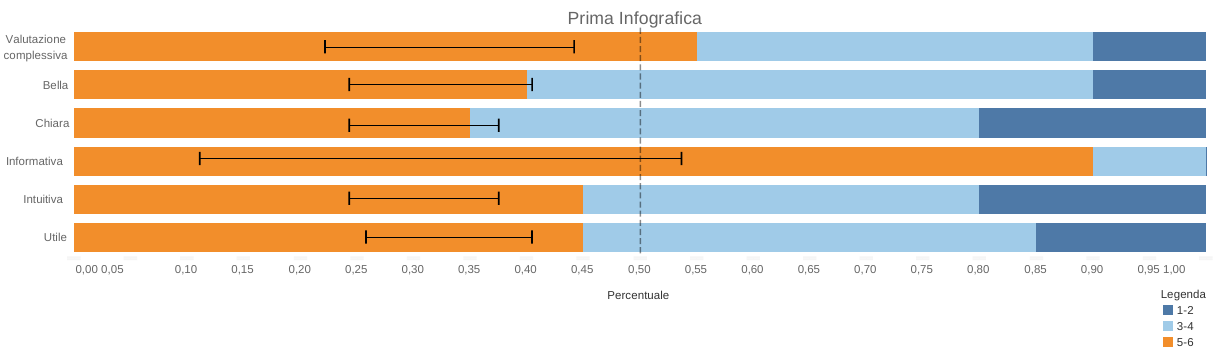
\includegraphics[width=1\linewidth]{imgs/vis1.png}
			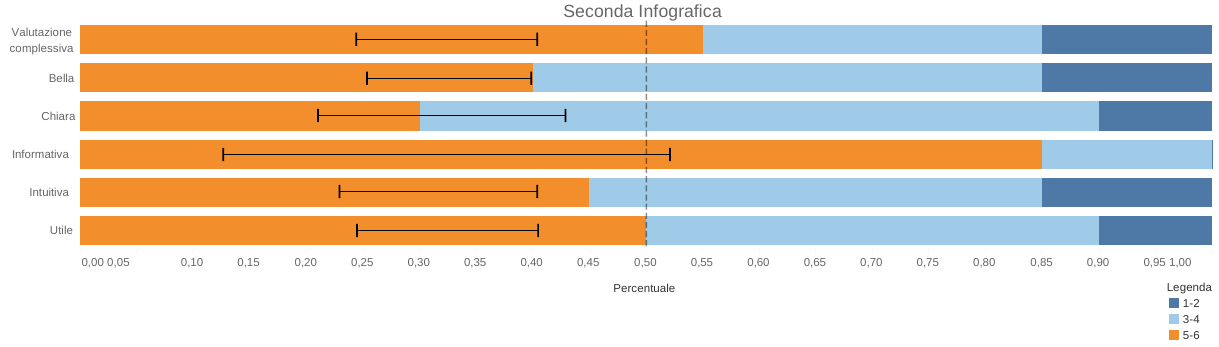
\includegraphics[width=1\linewidth]{imgs/vis2.png}
			\caption{Stacked barplot}
			\label{fig:Terza infografica1}
		\end{figure}
Gli stacked bar plot riferiti alle prime due infografiche mostrano risultati interessanti. Possiamo infatti notare come per entrambi l'intervallo di confidenza per la voce \textit{Informativa} includa il valore 0.5. Da ciò si può concludere che tale maggioranza non è significativa e pertanto non può rappresentare il giudizio dell'intera popolazione. Viceversa per la voce \textit{Valutazione Complessiva} il giudizio fornito dalla maggioranza risulta significativo quindi potrebbe essere rappresentativo dell'intera popolazione. 
\newpage

\begin{figure}[h]
			\centering
			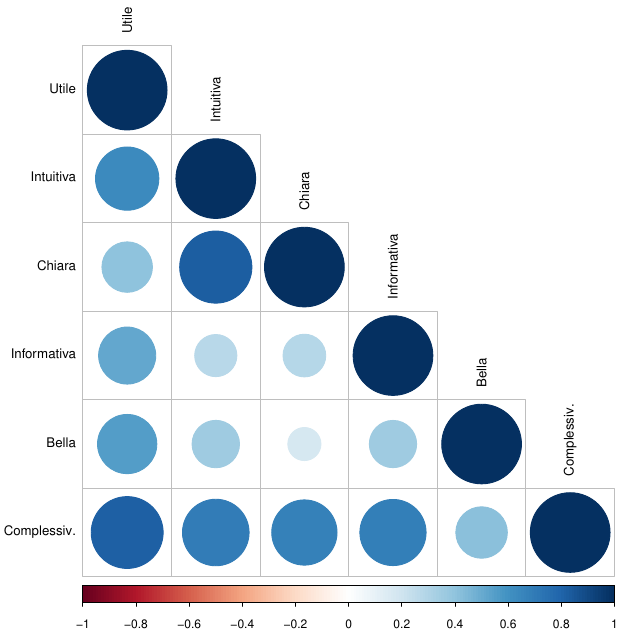
\includegraphics[width=0.4\linewidth]{imgs/corrVIS1.png}
			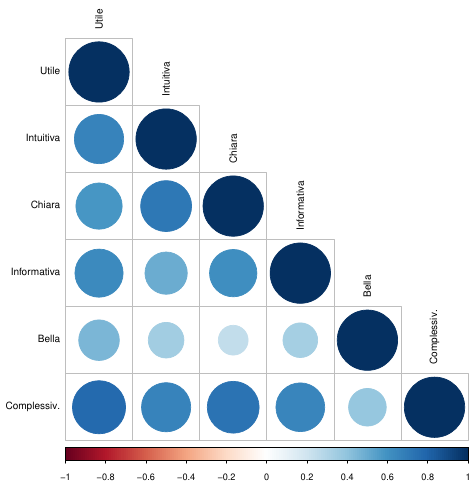
\includegraphics[width=0.4\linewidth]{imgs/corrVIS2.png}
			\caption{Correlogramma Prima Infografica (sx) e Seconda Infografica (dx)}
			\label{fig:Terza infografica1}
		\end{figure}
		

Dai correlogrammi si può invece notare un'alta correlazione fra le voci \textit{Intuitiva} e \textit{Chiara} e fra \textit{Complessiva} e \textit{Utile}, meno accentuata è invece la correlazione fra \textit{Intuitiva} e \textit{Utile} e fra \textit{Complessiva} e le voci: \textit{Intuitiva}, \textit{Chiara} e \textit{Informativa}. Molto bassa risulta inoltre la correlazione tra \textit{Bella} e le altre voci per entrambe le infografiche, sintomo del fatto che per queste due hanno prevalso altre qualità sulla bellezza come l'informatività e l'utilità.


\subsection{Terza e quarta infografica}

	\begin{figure}[h]
			\centering
			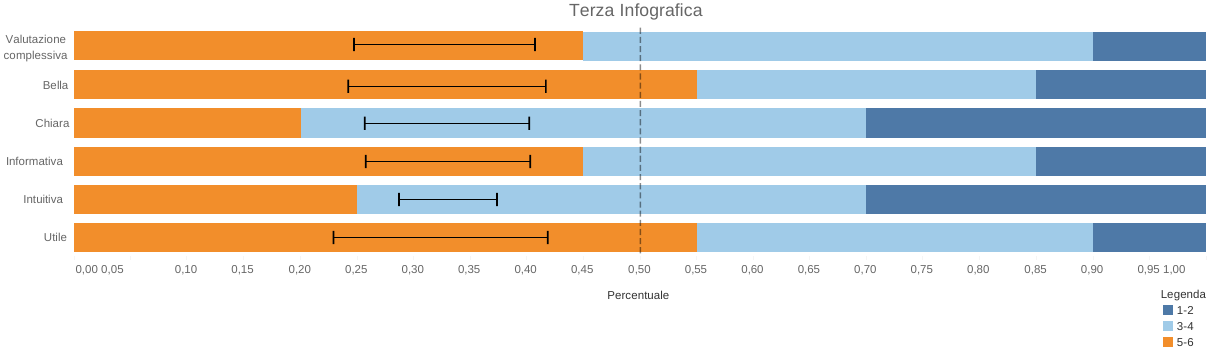
\includegraphics[width=1\linewidth]{imgs/vis3.png}
			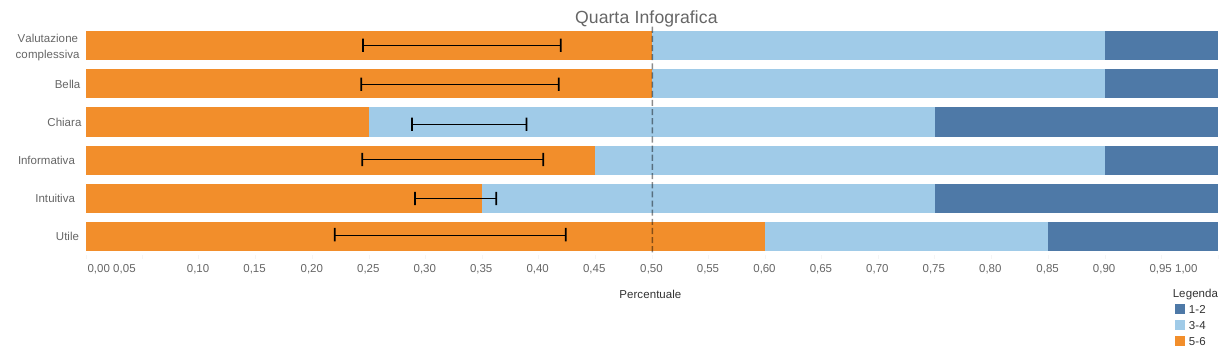
\includegraphics[width=1\linewidth]{imgs/vis4.png}
			\caption{Stacked barplot}
			\label{fig:Terza infografica11}
		\end{figure}

Gli stacked bar plot riferiti alla terza e quarta infografica mostrano invece la presenza di una maggioranza significativa rispettivamente per le voci \textit{Bella} e \textit{Utile} e per la voce \textit{Utile}.  

\begin{figure}[h]
			\centering
			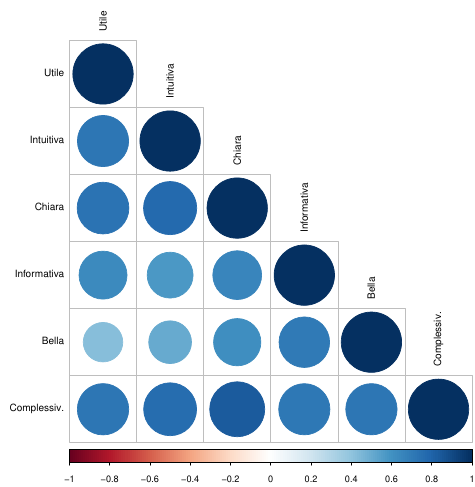
\includegraphics[width=0.4\linewidth]{imgs/corrVIS3.png}
			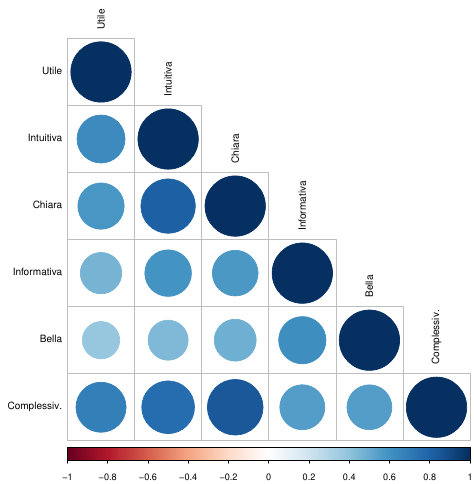
\includegraphics[width=0.4\linewidth]{imgs/corrVIS4.png}
			\caption{Correlogramma Terza Infografica (sx) e Quarta Infografica (dx)}
			\label{fig:Terza infografica111}
		\end{figure}

\newpage
Mentre dai correlogrammi si può notare che vi è un'alta correlazione fra la voce \textit{Complessivamente} e le voci \textit{Utile}, \textit{Intuitiva} e \textit{Chiara} e ancora fra \textit{Chiara} e \textit{Utile}, fra \textit{Chiara} e \textit{Intuitiva}. Per entrambe le infografiche risulta più debole la correlazione fra \textit{Bella} e \textit{Utile} e fra \textit{Bella} e \textit{Intuitiva}. Molto probabilmente per tali infografiche prevale la chiarezza, l'intuitività e l'utilità sulla bellezza. 

\subsection{Quinta infografica}

	\begin{figure}[h]
			\centering
			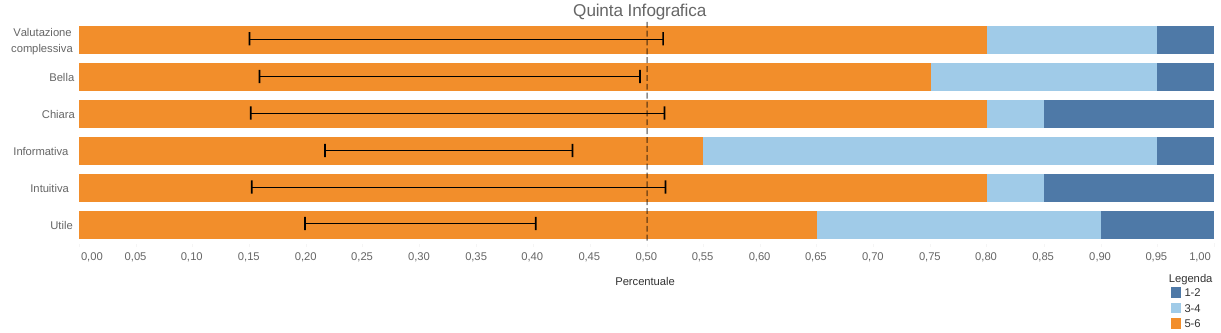
\includegraphics[width=1\linewidth]{imgs/vis5.png}
			\caption{Stacked barplot}
			\label{fig:Terza infografica11}
		\end{figure}
Infine per la quinta infografica, per le voci: \textit{Valutazione Complessiva}, \textit{Chiara} e \textit{Intuitiva} la maggioranza non risulta significativa, mentre risulta significativa la maggioranza relativa alle voci \textit{Bella}, \textit{Informativa} e \textit{Utile}. 	Rispetto alle infografiche precedenti questa viene ritenuta particolarmente bella e utile.  

\newpage

\begin{figure}[h]
			\centering
			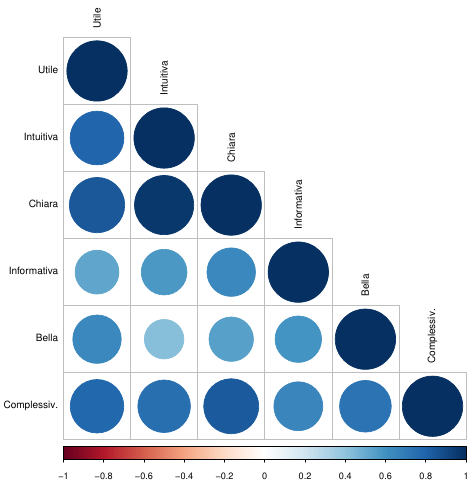
\includegraphics[width=0.4\linewidth]{imgs/corrVIS5.png}
			\caption{Correlogramma Quinta Infografica}
			\label{fig:Terza infografica111}
		\end{figure}


Nell'ultimo correlogramma è possibile notare un'altissima correlazione fra le voci \textit{Chiara} e \textit{Intuitiva}, ciò suggerisce che l'ultima visualizzazione è più intuitiva rispetto alle precedenti, dove infatti la correlazione rispetto alle stesse voci risultava inferiore. 

\newpage
\section{User test}

Ad un campione di 10 soggetti è stato richiesto di svolgere cinque task che prevedevano l'interazione con le infografiche tenendo conto del tempo impiegato per rispondere. Ciò è stato fatto al fine di comprendere se le informazioni che volevamo trasmettere tramite le infografiche erano facilmente comprensibili.

I cinque task che sono stati sottoposti sono i seguenti: 
\begin{enumerate}
    \item Nelll'infografica 1, a quale film è associato il picco più alto di tweet?
    \item Nell'infografica  1, quale film ha vinto nella categoria “Best Picture"? Nell'infografica  2 quale attore/attrice ha vinto nella categoria “Actress in a supporting role"?
    \item Nella infografica 3 quale film ha ottenuto un “Rating TMDB" maggiore?
\item Nella infografica 4 chi è stato più discusso durante la serata (ha ottenuto più tweet complessivamente)?
\item A quale categoria appartengono i film meno discussi durante la serata?
\end{enumerate}
\begin{figure}[h]
			\centering
			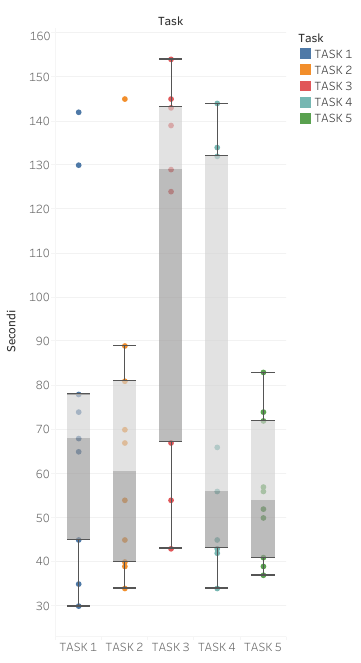
\includegraphics[width=0.4\linewidth]{imgs/User test.png}
			\caption{Box-plot user test}
			\label{fig:Terza infografica111}
		\end{figure}

Dal box-plot emerge che per task 1, 2 e 5 i tempi medi variano tra i 30 e i 90 secondi. Particolare invece risulta la situazione per i task 3 e 4 dove per il task 3 i tempi risultano visibilmente aumentati fino a superare i 120 secondi con la presenza di alcuni tempi molto bassi viceversa per il task 4 i tempi sono visibilmente bassi con la presenza di alcuni tempi molto alti.  

\paragraph{Link all'infografica}
\begin{verbatim}
https://public.tableau.com/views/DataVizProject_16311111989820/Storia1?
:language=it-IT&publish=yes&:display_count=n&:origin=viz_share_link
\end{verbatim}
\bibliographystyle{ieeetr}
% Importa il file bibliography.bib
\bibliography{bibliography}
\end{document}
